\documentclass[9pt]{beamer}
\usetheme[progressstyle=movCircCnt]{PBEsimple}

\usepackage[T1]{fontenc}
\usepackage[utf8]{inputenc}
\usepackage[portuguese]{babel}
\usepackage{animate}
\usepackage{multicol}
\usepackage{amsfonts}
\usepackage{amssymb}
\usepackage{multirow}
\usepackage{array,booktabs}
\newcommand{\PR}[1]{\ensuremath{\left[#1\right]}}
\newcommand{\PC}[1]{\ensuremath{\left(#1\right)}}
\newcommand{\chav}[1]{\ensuremath{\left\{#1\right\}}}

\title[Bioestatística]{\bf Bioestatística\\
\vspace{.3\baselineskip}}
\subtitle[]{\bf}

\date{ 30 de Março de 2017}
\author[Isolde Previdelli]{
  Isolde Previdelli\\
  \href{itsprevidelli@uem.br}{{\tt itsprevidelli@uem.br \\
isoldeprevidelli@gmail.com \\ \vspace{8mm} \tt \textbf{\LARGE{AULA 6 -
    Variáveis aleatórias}}}}
}
\institute[PBE/UEM]{}

% % % % % % % % % % % % % % % % % % % % % % % % % % % % % % % % % %

\begin{document}
% Página Título
{\pbebg
\begin{frame}[plain,noframenumbering]
  \titlepage
\end{frame}}

%%%%%%%%%%%%%%
\begin{frame}{Sumário}{}
\tableofcontents
\end{frame}
%%%%%%%%%%%%%%

\section{Variável Aleatória}
%\subsection{Etapas na análise de dados}

\begin{frame}{Variável aleatória}{}

%\begin{block}{red}{Definição}
\begin{itemize}
\item $X:\Omega \rightarrow$ é variável aleatória se o evento $[X \leq x] \in
\Lambda, \forall x \in \mathbb{R}$, tal que:
\item $X^{-1}(I) = \{\omega \in \Omega : X(\omega) \in I\} \in \Lambda$,
  em outras palavras, X é tal que sua imagem inversa de intervalos
$I \subset$ pertencem a $\sigma-$álgebra $\Lambda$.
\item A função $x(\omega)$ associa a cada evento em $\Omega$ um número real.
\item Variável aleatória é uma função do espaço amostral $\Omega$
  nos reais, para qual é possível calcular a probabilidade de ocorrência
  de seus valores.
\end{itemize}
%\end{block}

\begin{figure}[!htb]
    \centering
   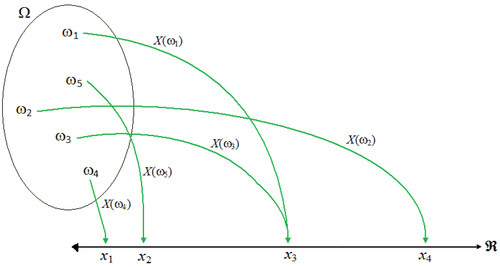
\includegraphics[scale=0.55]{va.png}
  \end{figure}
\end{frame}


%\subsection{Variável aleatória discreta}
\begin{frame}{Variável aleatória}{}

\begin{block}{red}{Variável aleatória discreta}
\begin{itemize}
\item Seu campo de variação é um conjunto finito ou infinito enumerável.
\item Para cada valor assumido existe uma certa probabilidade de ocorrência.
\end{itemize}
\end{block}

%Exemplo: lançamento de dois dados:

%\begin{figure}[!htb]
%    \centering
%   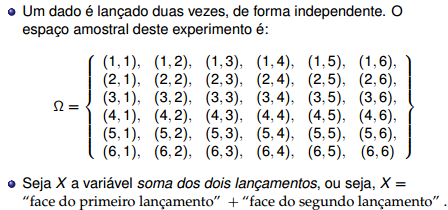
\includegraphics[scale=0.55]{ex_dados.png}
%  \end{figure}

%\end{frame}

\begin{block}{red}{Variável aleatória contínua}
\begin{itemize}
\item Seu campo de variação é um conjunto infinito(indeterminado) não-
enumerável.
\item A probabilidade e definida como a área entre dois pontos a e b.
\end{itemize}
\end{block}
\end{frame}

\subsection{Função de distribuição}
\begin{frame}{Função de distribuição}{}

A função de distribuição é útil pois permite
obter qualquer informação sobre a variável aleatória:


\begin{block}{red}{Definição}{}
\begin{itemize}
\item $F_x(x) = P(X \in (-\infty, x]) = P(X \leq x)$
\end{itemize}
\end{block}

\begin{block}{red}{Propriedades}{}
\begin{itemize}
\item (F1) $\lim_{n \to -\infty}F(x) = 0$ e $\lim_{n \to \infty} F(x) =
  1$;
\item (F2) $F$ é contínua à direita;
\item (F3) $F$ é não decrescente, isto é, $F(x) \leq F(y)$ sempre que $x
  \leq y, \forall x, y \in \mathbb{R}$.
\end{itemize}
\end{block}

\end{frame}

\subsection{Função de probabilidade e densidade de probabilidade}
\begin{frame}{Função de probabilidade}{}

\begin{block}{red}{Função de probabilidade(f.p.)}{}
\begin{itemize}
\item f.p. de uma variável aleatória discreta, representada por $P(X=x) =
p(x)$, é qualquer função tal que:

$X(\omega) \in \{x_1, x_2, ...\}\forall \omega \in \Omega$, tem-se, $p(x_i) \geq 0$ e $\displaystyle{
\sum_{i=1}^\infty p(x_i) = 1}$


\end{itemize}
\end{block}


\begin{block}{red}{Função densidade de probabilidade(f.d.p.)}{}
\begin{itemize}
\item f.d.p. de uma variável aleatória contínua, representada por
  $f_x(x)$
é qualquer função tal que:

$f_x(x) \geq 0$ e $\displaystyle{\int_{-\infty}^{\infty} f(x)_xdx = 1}$


\end{itemize}
\end{block}
\end{frame}


\subsection{Esperança matemática}
\begin{frame}{Esperança matemática}{}
\begin{itemize}
\item \textbf{A esperança matemática de uma variável aleatória é usualmente
referida como uma medida de posição da distribuição dessa variável.}
\item \textbf{Valor esperado, pondera os valores assumidos da variável aleatória
  pelas respectivas probabilidades.}
\item \textbf{É calculada para variáveis aleatórias discretas e contínuas.}
\end{itemize}

\end{frame}


\begin{frame}{Esperança matemática}{}

\begin{block}{blue}{Definição}
Seja $X$ uma variável aleatória \textbf{discreta}, a esperança
matemática é:

$$\mu = E(x) = \displaystyle{\sum_{i=1}^n}x_iP_x(x) =
\displaystyle{\sum_{i=1}^n} x_i P(X=x_i)$$

\end{block}

\end{frame}

\begin{frame}{Esperança matemática}{}

\begin{block}{blue}{Definição}
Seja $X$ uma variável aleatória \textbf{contínua}, a esperança
matemática é:

$$\mu = E(x) = \displaystyle{\int_{-\infty}^\infty}xf_x(x)$$

\end{block}

\end{frame}


\begin{frame}{Propriedades da esperança matemática}{}

\begin{block}{blue}{Propriedades}
\begin{itemize}
\item A esperança de uma constante é a própria constante: $E(K) = K$.
\item Multiplicando uma variável aleatória $X$ por uma constante,
sua esperança fica multiplicada por essa constante: $E(KX) = KE(X)$.
\item A esperança da soma ou da diferença de duas variáveis aleatórias é
igual a soma ou diferença das esperanças: $E(X \pm Y) = E(X) \pm E(Y)$.
\item Somando ou subtraindo uma constante a uma variável aleatória,
a esperança fica somada ou subtraída por essa constante:
$E(X \pm K) = E(X) \pm K$.
\item A esperança do produto de duas variáveis aleatórias com
distribuição conjunta $P(x, y)$, será o produto das esperanças,
sempre que as variáveis aleatórias forem independentes:
$ E(XY) = E(X)E(Y)$.
\end{itemize}

\end{block}

\end{frame}

\subsection{Variância}
\begin{frame}{Variância}{}

\begin{block}{blue}{Definição}
Seja $X$ uma variável aleatória \textbf{discreta}, a sua variância é:

$$\sigma^2 = Var(x) = E[X-\mu]^2 = E(x^2) - [E(x)]^2$$
onde, $E(x^2) = \displaystyle{\sum_{i=1}^n}x_i^2P(X=x_i)$

\end{block}

\end{frame}

\begin{frame}{Variância}{}

\begin{block}{blue}{Definição}
Seja $X$ uma variável aleatória \textbf{contínua}, a sua variância é:

$$\sigma^2 = Var(x) = E[X- \mu]^2 =
\displaystyle{\int_{-\infty}^\infty}(x - \mu)^2f_x(x)dx$$

\end{block}

\end{frame}


\begin{frame}{Propriedades da variância}{}

\begin{block}{blue}{Propriedades}
\begin{itemize}
\item A variância de uma constante é zero, $Var(K)=0$.
\item Multiplicando-se uma variável aleatória por uma constante sua
variância fica multiplicada pelo quadrado da constante, $Var(KX) =
K^2Var(X)$.
\item Somando-se ou subtraindo-se uma constante à variável aleatória,
sua variância não se altera, $Var(K \pm X) = Var(X)$
\item A variância da soma ou da diferença de duas variáveis aletórias é:
$V(X \pm Y) =  Var(x) + Var(Y) \pm 2 cov(X,Y)$, em que $cov(X,Y) = E(XY)-E(X)E(Y)$
\end{itemize}

\end{block}

\end{frame}



%%%%%%%%%%%%%%%

{\pbebg
\begin{frame}[plain,noframenumbering]

\finalpage{\begin{figure}[!htb]
    \centering
   
\includegraphics[scale=0.475]{probII.jpg}
  \end{figure}
Obrigada!}

\end{frame}}
%%%%%%%%%%%%%%%%
\end{document}